\documentclass[tikz, border=5pt]{standalone}

\begin{document}
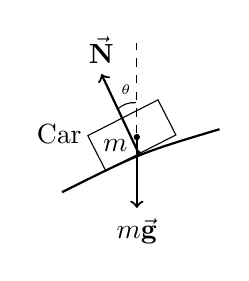
\begin{tikzpicture}

    %% FBD of the car

    % Car
    \begin{scope}[rotate=27]
        \draw (-0.5, 0) rectangle (0.5, 0.5);
        \node [left] at (0, 0.1) {\( m \)};
        \node [left] at (-0.45, 0.5) {Car};
    \end{scope}

    % Ground
    \draw[thick] (-1, -0.5) .. controls (0,0) .. (1, 0.3);

    % Reference line
    \draw[dashed] (-0.05, 0.25) -- (-0.05, 1.4);

    % Angle
    \draw (-0.30, 0.55) arc[start angle=135, end angle=85, radius=0.3] node[pos=0.5, above] {\tiny \( \theta \)};

    % Normal reaction force
    \draw[thick, ->] (-0.03, 0) -- (-0.5, 1) node[above] {\( \vec{\mathbf{N}} \)};
    \fill (-0.03, 0) circle (0.03);

    % Gravitational force
    \draw[thick, ->] (-0.05, 0.2) -- (-0.05, -0.7) node[below] {\( m\vec{\mathbf{g}} \)};
    \fill (-0.05, 0.2) circle (0.04);

\end{tikzpicture}
\end{document}
